\chapter{Background}

%%%%%%%%%%%%%%%%%   SECTION : INTRODUCTION   %%%%%%%%%%%%%%%%%%%%%%%%%%%%%%
\section{Introduction} \label{what is moo}
In today's increasingly complex world, decision makers often face the challenge of optimizing several conflicting objectives simultaneously. \acrfull{moo} 
is an optimization that deals with such problems, where multiple objective functions are optimized simultaneously. A detailed understanding of \acrshort{moo} 
is provided in the following sections.

\paragraph{Example:}
A car consists of many components like engine, body, wheels and many more which can be
tweaked. In this example, the manufacturer wants to optimize the car for two objectives: lower manufacturing cost of the car and lower carbon emissions. With 
considering the input parameters and the objectives, many solution are obtained as shown in Figure \ref{moo}

\begin{figure}[!h]
	\begin{center}
		\input{../Python/plots/moo_plot.tex}
	\end{center}
    \caption{Example of \acrshort{moo}}
    \label{moo}
\end{figure}
In an \acrshort{moo} problem, there typically is no single best solution. Rather, the \textit{goal} is to identify a set of solutions that are optimal in terms 
of all objectives. In Figure \ref{moo}, the best solutions for the given objectives is indicated in orange known as pareto optimal solutions. A solution is said 
to be pareto optimal if no other solution can improve on any of the objectives without worsening at least one of the other objectives\cite{Benson2009}.
%The solutions which are not Pareto optimal are not considered as they are dominated by the Pareto optimal solutions. 

\section{Difference between \acrlong{moo} and \acrlong{soo}}
Optimization problems, whether single-objective or multi-objective, have the same goal: to find the best solution(s) to a given problem. However, the approach
to solving these problems is different. 

In \acrfull{soo}, the goal is to optimize a single objective function, which can either be maximized or minimized. The  problem is simpler to define and solve
because it involves only one objective. To calculate \acrshort{soo}, methods like gradient descent, linear programming and many more are used.

\begin{figure}[!h]
    \centering
    \input{../Python/plots/soo_plot.tex}
    \caption{Example of \acrshort{soo}}
    \label{soo}
\end{figure}

In Figure \ref{soo}, the same example given in Section \ref{what is moo} is considered. But, here, the manufacturer considers only \textbf{one objective}, minimizing 
the manufacturing cost. This is shown in the y-axis. The best solution is highlighted in orange.

In \acrshort{moo}, the optimization involves two or more objective functions simultaneously. The problem is more complex because the objectives are often
conflicting. Unlike \acrshort{soo}, where a single best solution is obtained, in \acrshort{moo}, pareto optimal solutions are obtained.
To calculate \acrshort{moo}, methods like pareto optimization, scalarization method, weighted sum method, $\epsilon$-constraint method, etc are used.


While \acrshort{soo} focuses on finding the best solution according to a single criterion, \acrshort{moo} addresses the more complex task of balancing multiple, 
often conflicting objectives. The choice between \acrshort{soo} and \acrshort{moo} depends on the nature of the problem at hand and the goals of the decision-maker. 
Understanding the differences between these approaches is crucial for selecting the appropriate optimization technique and achieving the desired outcomes.

%%%%%%%%%%%%%%%   SECTION : OPTISLANG  %%%%%%%%%%%%%%%%%%%%%%%%%%%%%%%%
\section{Softwares used for \acrlong{moo}}
\paragraph{}

To calculate \acrshort{moo}, a software platform which can handle the complexity of the problem is required. Ansys Optislang \cite{optislang} is one such software,  
which is used for design exploration, \acrfull{cae} based sensitivity analysis and optimization in conjunction with any product development tool. 
It is a Process Integration and Design Optimization tool or in short, a \acrshort{pido} tool. Process Integration refers to automate and orchestrate manual 
simulation processes and to realize complex workflows. Design Optimization aims for better understanding of your design, optimizing the product, identify an 
improved design which has the desired qualities and resulting in a best design by reliability analysis and statistical analysis.  


Optislang uses several solvers to look into aspects like mechanical, technical, mathematical and any other problems. This is easier in Optislang as it provides
integration to create toolchains of many external programs like ANSYS, MATLAB, Excel, Python, CATIA and many more. Our department utilizes Optislang for solving 
\acrshort{moo} problems, as it includes algorithms specifically designed for it. System developers design the modules and later integrate them into Optislang 
as a parametric system. Parametric system refers to a simulation model is defined using parameters which can be varied. By adjusting the parameters, the 
simulation model can be used to explore the behavior of the system under different conditions. Apart from \acrshort{moo}, Optislang can also be used for 
sensitivity analysis, robustness analysis, reliability analysis, and many more. 
%# Try to explain about the parametric system, sensitivity analysis, MOP, ...
%%%%%%%%%%%%%%%%%   SECTION : MODULES AND WORKFLOWS   %%%%%%%%%%%%%%%%%%%%%%%%%%%%%%
\section{Modules and Workflows}
\subsection{Modules}
Modules are created by the system developers. Modules include a simulation model as a calculation with defined interfaces for coupling with other modules. 
These modules are either defined in MATLAB or Python. Each module is designed to tackle a specific issue. To document and collaborate with other
system developers, every module is versioned and stored in a specific manner in a repository in GitHub Enterprise. Figure \ref{github_arrhenius} shows the 
structure of how each module is maintained in GitHub organization.

%!Crop the image to it's normal size
\begin{figure}[!ht]
    \centering
    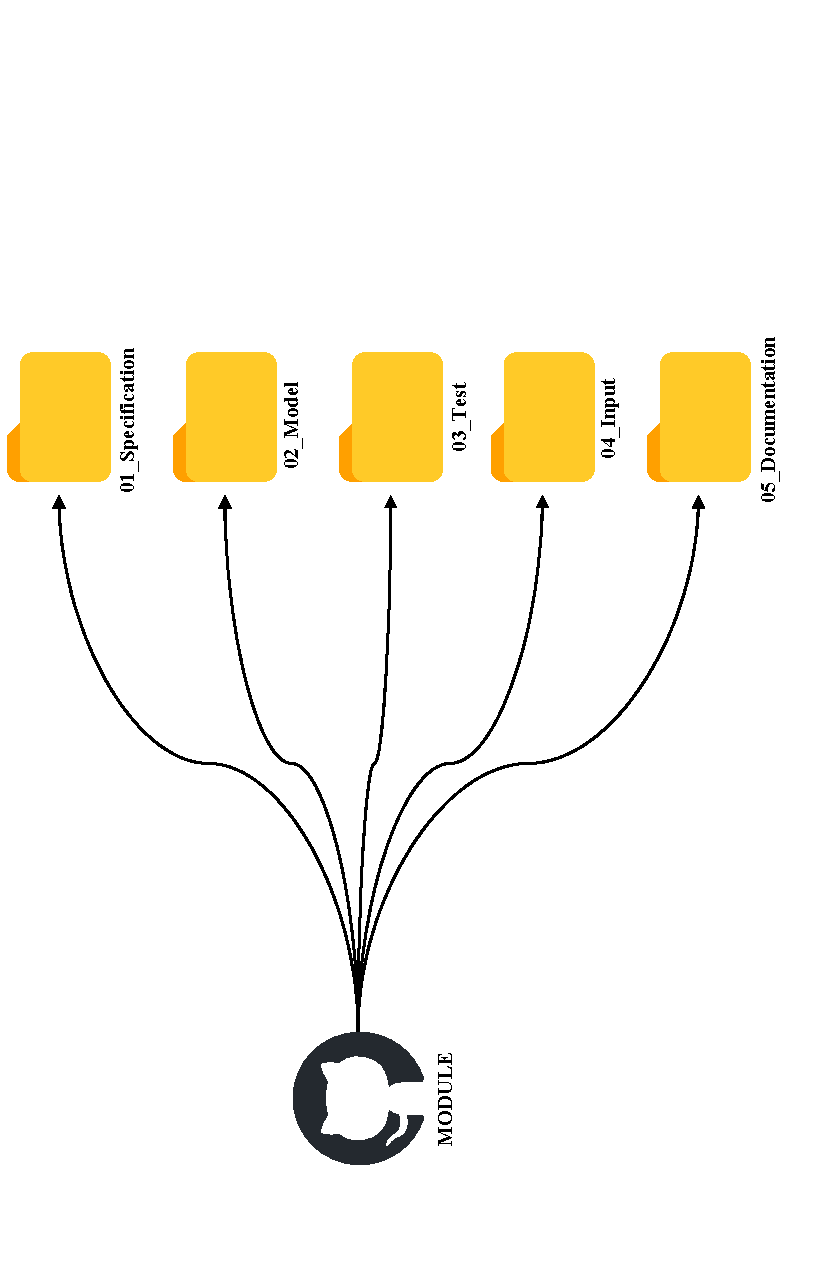
\includegraphics[width=0.63\textwidth, angle=-90]{Images/github_folder_structure_2.pdf}
    \caption{Structure of a module in GitHub Enterprise}
    \label{github_arrhenius}
\end{figure}
\newpage
\begin{itemize}
    \item \verb|01_Specification| has all the requirements for the module to run.
    \item \verb|02_Model| contains all parts to run the model. This can also be used as a playground for the development of a model.
    \item \verb|03_Test| contains all the unit tests for the module. This is to ensure that the module is working as expected.
    \item \verb|04_Input| carries all the initial parameters or functions to be defined at the start of a module.
    \item \verb|05_Documentation| contains documents explaining functioning and usage of the module.
\end{itemize}

\subsection{Workflows}
System developers at Bosch are responsible for developing automatized workflows for power electronics products considering functional loads, reliability indications and many more. Workflows 
are a sequence of modules designed for a fast calculation performance characteristic like temperature or reliability indication. To develop a workflow, 
Optislang is used. Every architectural workflow has a GitHub repository 
that is maintained in a similar way to how modules are being maintained. Figure \ref{workflow_example} shows an example of a workflow implemented in Optislang.
\begin{figure}[!h]
    \centering
    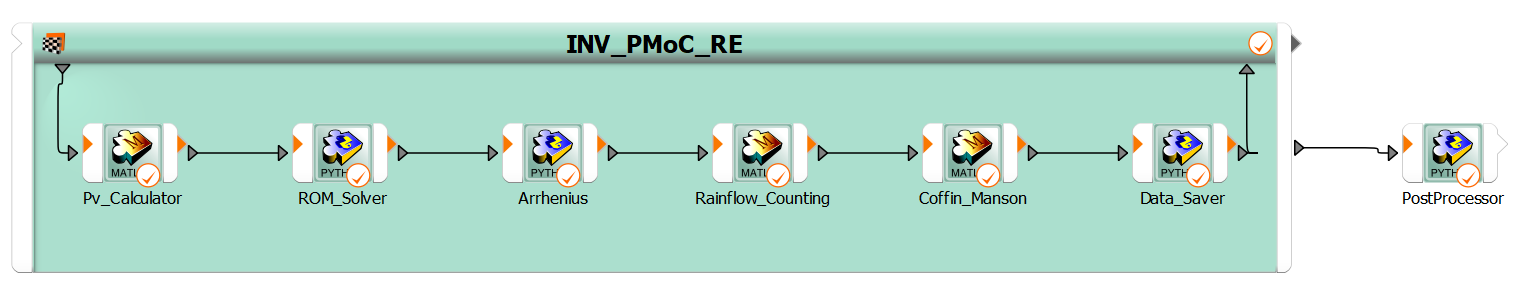
\includegraphics[width=\textwidth]{Images/workflow_example.png}
    \caption{Example of a workflow in Optislang}
    \label{workflow_example}
\end{figure}

In the above Figure \ref{workflow_example}, the workflow \texttt{INV\_PMoC\_RE} is responsible for providing fast, automatized and modular electro-thermal based 
reliability assessment and optimization for a Power Module on Cooler (PMoC). The workflow consists of several modules like \texttt{ARRHENIUS}, \texttt{ROM SOLVER},
\texttt{PV CALCULATOR} and many more.
\subsection*{}
For workflows and modules, the department follows a quality assurance process called \textbf{Model Readiness Level (MRL)}. Higher the readiness level, higher
the maturity of the module or workflow. This quality assurance process ensures that the modules and workflows are not developed for a small development 
circle, but for a broader audience. It also ensures that the modules and workflows are well documented, tested and maintained.

%%%%%%%%%%%%%%%%%   SECTION : CURRENT PROBLEM   %%%%%%%%%%%%%%%%%%%%%%%%%%%%%%
\section{Current Problems} \label{current problem}
There are several modules and workflows developed by the system developers at Bosch. While introducing a new feature or fixing a bug, the developer needs to test their
newly implemented code locally. Later, they need to test their feature in Optislang to ensure the functionality of the module or workflow. This process is 
time demanding. Some of the module or workflow tests are complex considering the number of parameters, which makes the testing process error prone. Currently, 
developers are spending a significant amount of time testing the modules and workflows. This is not a sustainable solution considering the fast-paced development in the automotive industry.

Every system developer or a team of system developers is responsible for developing the modules and workflows. Each module or workflow is developed in a 
specific way. Some of the older modules are maintained with different standards than the newer ones. This leads to a lack of standardization 
in the modules and workflows. This lack of standardization makes it difficult to maintain the modules and workflows 
effectively.\newline

Considering the above problems, developing a digitalization strategy for automated development of a module or workflow is a key point to keep Bosch competitive 
in a constantly evolving market where a fast, reliable and sustainable product development is crucial.